% ------------------------------------------------------------------------------
% TYPO3 Version 10 LTS - What's New (English Version)
%
% @author	Michael Schams <schams.net>
% @license	Creative Commons BY-NC-SA 3.0
% @link		https://typo3.org/help/documentation/whats-new/
% @language	English
% ------------------------------------------------------------------------------

\section{Inleiding}
\begin{frame}[fragile]
	\frametitle{Inleiding}

	\begin{center}\huge{\color{typo3darkgrey}\textbf{Inleiding}}\end{center}
	\begin{center}\large{\textit{Belangrijke feiten over TYPO3 v10 LTS}}\end{center}

\end{frame}

% ------------------------------------------------------------------------------
% TYPO3 Version 10 LTS - The Facts

\begin{frame}[fragile]
	\frametitle{Inleiding}
	\framesubtitle{TYPO3 Versie 10 LTS}

	\begin{itemize}
		\item Publicatiedatum: 21 april 2020
		\item Publicatietype: LTS (long-term support)
	\end{itemize}

	\begin{figure}
		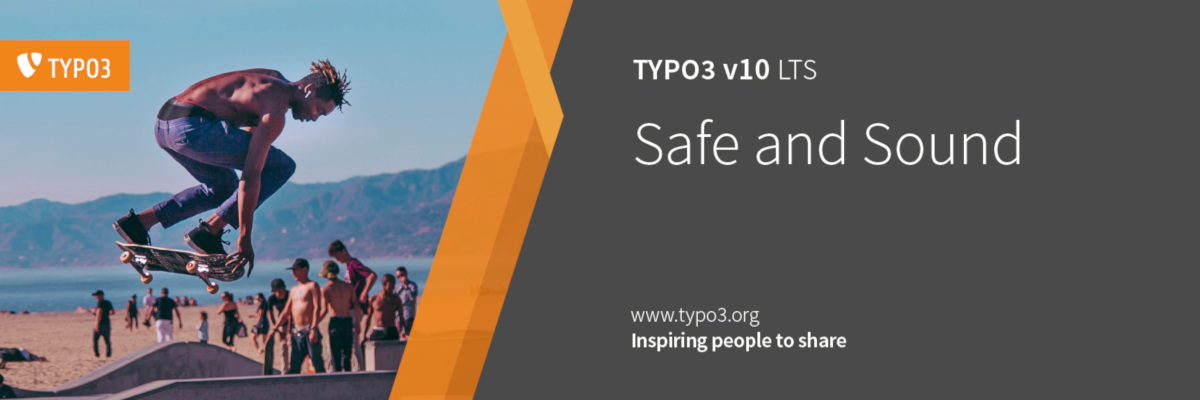
\includegraphics[width=0.95\linewidth]{Introduction/typo3-v10-4-banner.jpg}
	\end{figure}

\end{frame}

% ------------------------------------------------------------------------------
% TYPO3 Version 10 LTS - Executive Summary

\begin{frame}[fragile]
	\frametitle{Inleiding}
	\framesubtitle{Managementsamenvatting}

	\small
		TYPO3 v10.4 (ook TYPO3 v10 LTS genoemd om aan te geven dat de long-term support versie is)
		is het nieuwe vlaggenschip en, zonder twijfel, een van de meest geavanceerde op PHP gebaseerde OpenSource
		content management systemen op de markt op dit moment.

		\vspace{0.2cm}

		Na het publiceren van vijf sprintversies sinds juli 2019 kunnen we trots stellen dat we
		TYPO3 hebben uitgerust met de beste moderne PHP-bibliotheken en dat we enkele fantastische,
		nieuwe enterprise functies hebben toegevoegd.

		\vspace{0.2cm}

		Dit document vat de belangrijkste wijzigingen tussen TYPO3 v9 LTS en v10 LTS samen vanuit
		een technisch perspectief.

%		\vspace{0.2cm}
%
%		"What's New Slides" of all TYPO3 v10.x releases are available at
%		\href{https://typo3.org/help/documentation/whats-new/}{typo3.org}.

% changelog
% what's new slides

	\normalsize

\end{frame}

% ------------------------------------------------------------------------------
% System Requirements

\begin{frame}[fragile]
	\frametitle{Inleiding}
	\framesubtitle{Systeemeisen}

	\begin{itemize}
		\item PHP versie 7.2, 7.3 of 7.4
		\item PHP instellingen:

			\begin{itemize}
				\item \texttt{memory\_limit} >= 256M
				\item \texttt{max\_execution\_time} >= 240s
				\item \texttt{max\_input\_vars} >= 1500
				\item compilatieoptie \texttt{-}\texttt{-disable-ipv6} moet \underline{niet} worden gebruikt
			\end{itemize}

			\item Vereiste PHP extensies:\newline
				\small
					filter, hash, openssl, pcre >= 8.38, session, SPL, standard,
					xml, zip and zlib
				\normalsize

		\end{itemize}

\end{frame}

% ------------------------------------------------------------------------------
% System Requirements

\begin{frame}[fragile]
	\frametitle{Inleiding}
	\framesubtitle{Systeemeisen}

	\begin{itemize}
		\item Webserver zoals Apache, Nginx, IIS, etc.
		\item Alle databaseservers die worden ondersteund door \textbf{Doctrine DBAL}
			werken ook met TYPO3. Bijvoorbeeld:
	\end{itemize}

	\begin{figure}
		
\includegraphics[width=0.70\linewidth]{Introduction/logo-databases.png}
	\end{figure}

	\begin{itemize}
		\item Minimum schijfruimte: 200 MB
		\item De backend ondersteunt alle moderne browsers zoals Microsoft Edge,
			Google Chrome, Firefox, Safari of elke andere compatibele browser.
	\end{itemize}

\end{frame}

% ------------------------------------------------------------------------------
% Sprint Releases

\begin{frame}[fragile]
	\frametitle{Inleiding}
	\framesubtitle{Ontwikkelingstijdlijn}

	Gebupliceerde Sprint Releases:
	\vspace{0.4cm}
	\begin{itemize}
		\item v10.0 \tabto{1.1cm}23-juli-2019\tabto{3.4cm}De weg vrijmaken voor spannende nieuwe concepten en API's
		\item v10.1 \tabto{1.1cm}01-okt-2019\tabto{3.4cm}Verbeterde routing en Site behandeling v2
		\item v10.2 \tabto{1.1cm}03-dec-2019\tabto{3.4cm}Fluid/Rendering Engine verbeteringen
		\item v10.3 \tabto{1.1cm}25-feb-2020\tabto{3.4cm}Feature Freeze
		\item v10.4 \tabto{1.1cm}21-apr-2020\tabto{3.4cm}LTS Versie (long-term support)
	\end{itemize}

\end{frame}

% ------------------------------------------------------------------------------
% LTS Support Timeline

\begin{frame}[fragile]
	\frametitle{Inleiding}
	\framesubtitle{Long-term Support}

	\begin{figure}
		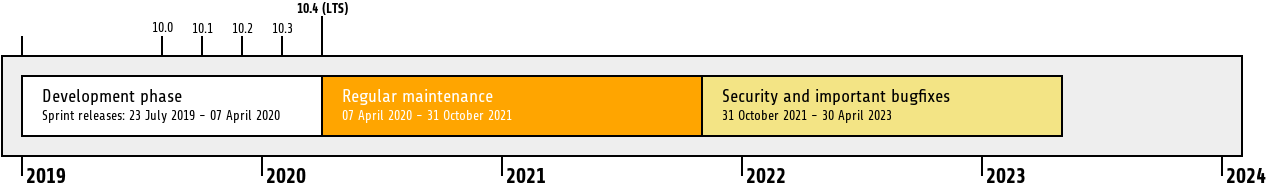
\includegraphics[width=1\linewidth]{Introduction/typo3-v10-lifecycle.png}
	\end{figure}

	\begin{itemize}
		\item TYPO3 version 10.4 is een LTS-versie (long-term support)
		\item Gewoon onderhoud en bugfixes tot oktober 2021
		\item Beveiligings- en kritische bugfixes tot april 2023
	\end{itemize}
	\vspace{0.2cm}
	\textbf{Verlengde ondersteuning}\newline
	\smaller
		\href{https://typo3.com}{TYPO3 GmbH} biedt verlengde long-term
			support (ELTS) voor TYPO3 v10 LTS tot april 2026.
	\normalsize

\end{frame}

% ------------------------------------------------------------------------------
